\documentclass[11pt,aspectratio=43,usenames,dvipsnames]{beamer}
\usepackage[utf8]{inputenc}
\usepackage{amsmath, amsfonts, amssymb, amsthm}
\usepackage[T1]{fontenc}
\usepackage{lmodern}
\usepackage{xcolor}
\usepackage{setspace}
\usepackage{booktabs}
\usepackage{multirow}
\usepackage{graphicx}
\usepackage{tikz}
% \usetikzlibrary{decorations}
\usetikzlibrary{decorations.pathreplacing, intersections}
\usepackage{ulem}
\usepackage{hyperref}
\usepackage{booktabs}
\usepackage{babel}
\usepackage{makecell}
\usepackage[para,online,flushleft]{threeparttable}
\usepackage{pdfpages}
\usepackage{tcolorbox}
\usepackage{bm}
\usepackage{appendixnumberbeamer}
\usepackage{natbib}
\usepackage{caption}
\captionsetup[figure]{labelformat=empty}% redefines the caption setup of the figures environment in the beamer class.
\usetheme[compress]{Boadilla}
\usecolortheme{default}
\useoutertheme{miniframes}
\usefonttheme[onlymath]{serif}

\newcommand{\jump}[2]{\hyperlink{#1}{\beamerbutton{#2}}}
\newcommand{\orange}[1]{\textcolor{BurntOrange}{#1}}
\newcommand{\red}[1]{\textcolor{red}{#1}}
\newcommand{\green}[1]{\textcolor{OliveGreen}{#1}}

\setbeamertemplate{itemize item}{\raisebox{0.1em}{\scalebox{0.7}{$\blacksquare$}}}
\setbeamertemplate{itemize subitem}[circle]
\setbeamertemplate{itemize subsubitem}{--}
\setbeamercolor{itemize item}{fg=black}
\setbeamercolor{itemize subitem}{fg=black}
\setbeamercolor{itemize subsubitem}{fg=black}
\setbeamercolor{item projected}{bg=darkgray,fg=white}
\definecolor{blue}{rgb}{0.2, 0.2, 0.7}
\setbeamercolor{alerted text}{fg=blue}
\setbeamertemplate{enumerate items}[circle]


\setbeamertemplate{headline}{}

%==========================================
\let\olditemize=\itemize
\let\endolditemize=\enditemize
\renewenvironment{itemize}{\olditemize \itemsep1em}{\endolditemize}
\let\oldenumerate=\enumerate
\let\endoldenumerate=\endenumerate
\renewenvironment{enumerate}{\oldenumerate \itemsep1em}{ \endoldenumerate}

\DeclareMathOperator*{\argmax}{\arg\!\max}
\DeclareMathOperator*{\E}{\mathbb{E}}
\DeclareMathOperator*{\var}{\rm Var}
\DeclareMathOperator*{\cov}{\rm Cov}

\theoremstyle{definition}
\newtheorem{assume}{Assumption}
\newtheorem{lem}{Lemma}
\newtheorem{proposition}{Proposition}
\newtheorem{thm}{Theorem}
\newtheorem{corol}{Corollary}

\begin{document}
    \title[Lecture 16]{Lecture 16 \\ The Real Business Cycle Model \\ Part 3: Competitive Equilibrium}
    \author[Hui-Jun Chen]{Hui-Jun Chen}
    \institute[OSU]{The Ohio State University}
    % \date{\today}
    \date{\today}
    \setbeamertemplate{navigation symbols}{}
    \setstretch{1.2}

%-------------------------------------------------------
{
%	\usebackgroundtemplate{\includegraphics[width=1\paperwidth]{../EveningSky_cropped_edit43_bright.jpg}}
    \begin{frame}
% \vspace{3em}
        \centering
%		{\footnotesize 	ECON 4002 Intermediate Macroeconomic Theory}
        \maketitle
% \vspace{-1.5em}
% \centering
% \includegraphics[width=0.55\linewidth]{Pictures/houses.jpeg}


    \end{frame}
}

% -------------------------------------------
\setbeamertemplate{headline}
{
\setbeamercolor{section in head/foot}{fg=black, bg=white}
\vskip1em \tiny \insertsectionnavigationhorizontal{1\paperwidth}{\hspace{0.50\paperwidth}}{}
}
%------------------------------------------


\begin{frame}{Overview}
\label{slide:Overview}
    \begin{itemize}
        \item Recall that in Lecture 13, there is no production in dynamic model.
        \item The following $ 5 $ lectures is for \textbf{Real Business Cycle} (RBC) model:
        \begin{itemize}
            \item Lecture 14: consumer
            \item Lecture 15: firm
            \item Lecture 16: competitive equilibrium
            \item Lecture 17: formal example
            \item Lecture 18: application to bring RBC to data
        \end{itemize}
    \end{itemize}
\end{frame}

\section{Complete the Model}
\label{sec:Complete_the_Model}

\begin{frame}{Review: Consumer's Problem}
\label{slide:Review__Consumer_Problem}
    Taken \alert{$\{ w, w', r, T, T', \pi, \pi' \}$} as given, a representative consumer chooses \green{$ \{ C', N_{S}, N'_{S} \} $} to solve
    %
    \begin{equation}
    \label{eq:consumer_problem}
        \begin{split}
            \max_{\green{C', N_{S}, N'_{S}}} \quad
                & u\left(
                    \alert{w} \green{N_{S}} + \alert{\pi} - \alert{T} + \frac{\alert{w'} \green{N'_{S}} + \alert{\pi'} - \alert{T'} - \green{C'}}{1+\alert{r}}
                   \right)
            \\
                & - v( \green{N_{S}} ) + u( \green{C'} ) - v( \green{N'_{S}} )
        \end{split}
    ,\end{equation}
    %
    which we can back out \green{$C, S, l, l'$}.
\end{frame}

\begin{frame}{Review: Firm's Problem}
\label{slide:Review__Firm_s_Problem}
    Taken \alert{ $ \{ w, w', r \} $} as given, a representative firm chooses \green{$\{ N_{D}, N'_{D}, K' \}$} to solve
    \begin{equation}
    \label{eq:firm_problem}
        \begin{split}
            \max_{\green{N_{D}, N'_{D}, K'}} \quad
                & z F( K, \green{N_{D}} ) - \alert{w} \green{N_{D}} - [ \green{K'} - ( 1-\delta )K ]
            \\
                & \qquad + \frac{z' F( \green{K'}, \green{N'_{D}} ) - \alert{w'} \green{N'_{D}} + ( 1-\delta ) \green{K'}}{1+\alert{r}}
            \\
        \end{split}
    ,\end{equation}
    which we can back out \green{$Y, Y', \pi, \pi', I$}
\end{frame}

\begin{frame}{Government Budget Constraint}
\label{slide:Government_Budget_Constraint}
    Government behaves exactly the same in two-period model:
    \begin{itemize}
        \item current budget constraint: $ G = T + B $
        \item future budget constraint: $G' + ( 1+r ) B = T'$
        \item lifetime budget constraint: $ \displaystyle G + \frac{G'}{1+\alert{r}} = \green{T} + \frac{\green{T'}}{1+\alert{r}} $
    \end{itemize}
    Taken \alert{$\{ r \}$} as given, government satisfy lifetime budget constraint by choosing \green{$\{ T, T', B \}$}.
\end{frame}

\begin{frame}{Market Clear}
\label{slide:Market_Clear}
    There are three markets to clear:
    \begin{enumerate}
        \item labor markets clear at each date determines wage:
        \begin{itemize}
            \item find $ w $ such that \green{$ N_{S} = N_{D} $ }
            \item find $ w' $ such that \green{$N'_{S} = N'_{D}$}
        \end{itemize}
        \item goods markets clear at each date determines consumption and investment:
        \begin{itemize}
            \item date $ 0 $ (today): $ \green{Y = C + I} + G $
            \item date $ 1 $ (tomorrow): $ \green{Y' = C' + I'} + G' $
        \end{itemize}
        \item bonds market clears at date $ 0 $ determines real interest rate:
        \begin{itemize}
            \item find $ r $ such that \green{$S = B$}
        \end{itemize}
    \end{enumerate}

\end{frame}

\begin{frame}{Competitive Equilibrium: RBC Model}
\label{slide:Competitive_Equilibrium__RBC_Model}
Given exogenous quantities \orange{$\{ G, G', z, z', K \}$}, a \textbf{competitive equilibrium} is a set of
\begin{columns}
    \begin{column}{0.5\textwidth}
        \begin{enumerate}
            \item consumer choices \green{$\{ C, C', N_{S}, N'_{S}, l, l', S \}$},
            \item firm choices \green{ $ \{ Y, Y', \pi, \pi', N_{D}, N'_{D}, I, K' \} $},
            \item government choices \green{ $ \{ T, T', B \} $}, and
            \item prices \green{ $ \{ w, w', r \} $}
        \end{enumerate}
        such that
    \end{column}
    \begin{column}{0.5\textwidth}
        \begin{enumerate}
            \item consumer solves problems in \eqref{eq:consumer_problem},
            \item firm solves problems in \eqref{eq:firm_problem},
            \item government balances its budget, and
            \item all three markets clear.
        \end{enumerate}
    \end{column}
\end{columns}
\end{frame}

\begin{frame}{Plan to analyze the Model}
\label{slide:Plan_to_analyze_the_Model}
    In the following slides, we are going to use graphical analysis on \alert{two markets} in \alert{current period}:
    \begin{enumerate}
        \item \alert{current labor market}: interaction of firm and consumer today
        \begin{itemize}
            \item similar to static model: \alert{labor supply} and \alert{labor demand} curves
            \item what's new: both curves reflect the dynamic tradeoff through interest rate
        \end{itemize}
        \item \alert{current goods market}: interaction of firm, consumer and government today
        \begin{itemize}
            \item new: construct and analyze \alert{output supply} and \alert{output demand} curves
        \end{itemize}
    \end{enumerate}
\end{frame}

\section{Work with Model}
\label{sec:Work_with_Model}

\begin{frame}{The Current Labor Market}
\label{slide:The_Current_Labor_Market}
    \begin{columns}
        \begin{column}{0.5\textwidth}
            \begin{center}
                \scriptsize
                Figure 11.14  Determination of Equilibrium in the Labor Market Given the Real Interest Rate $r$
            \end{center}

            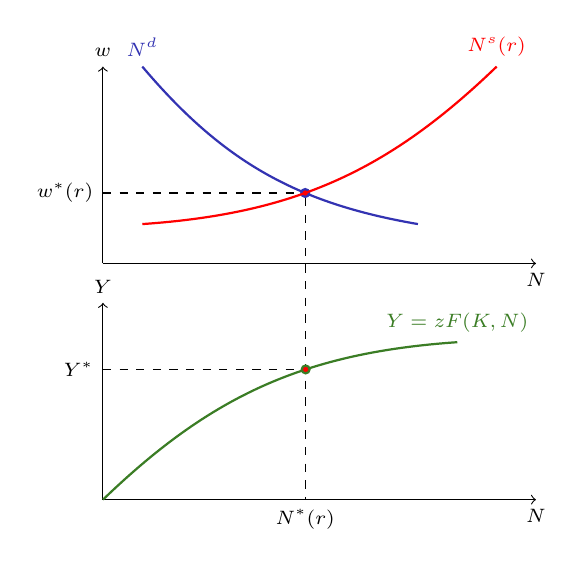
\begin{tikzpicture}
                \tikzstyle{every node}=[font=\scriptsize]
                \pgfmathsetmacro{\x}{5};
                \pgfmathsetmacro{\y}{2.5};
                % \draw[very thin,color=gray, step=0.1] (0,0) grid (\x, \y); % gray grid
                \draw[->, yshift = 3cm] (0,0) -- (\x + 0.5,0) node[below]{$N$} ;   % label x axis
                \draw[->, yshift = 3cm] (0,0) --  (0,\y) node[above]{$w$} ;   % label y axis
                \draw[thick, blue, yshift = 3cm]
                    (0.5, \y)
                    node[above]{$N^{d}$}
                    to[bend right=20]
                    node[pos=0.65,draw,fill=red,circle,inner sep=1pt] (a) {}
                    (4, 0.5);
                \draw[thick, red, yshift = 3cm]
                    (\x, \y)
                    node[above]{$N^{s}( r )$}
                    to[bend left=20]
                    (0.5, 0.5);
                \path (a); \pgfgetlastxy{\xcoord}{\ycoord};
                \coordinate (a_x) at (\xcoord, 0);
                \coordinate (a_y) at (0, \ycoord);

                \draw[dashed] (a_y) node[left]{$w^{*}( r )$} -- (a) -- (a_x) node[below]{$N^{*}( r )$};

                \draw[->] (0,0) -- (\x + 0.5,0) node[below]{$N$} ;   % label x axis
                \draw[->] (0,0) --  (0,\y) node[above]{$Y$} ;   % label y axis
                \draw[thick, OliveGreen]
                    (0, 0)
                    to[bend left=20]
                    node[pos=0.62,draw,fill=red,circle,inner sep=1pt] (b) {}
                    (\x-0.5, \y-0.5)
                    node[above]{$Y = zF(K, N)$};
                \path (b); \pgfgetlastxy{\xcoord}{\ycoord};
                \coordinate (b_x) at (\xcoord, 0);
                \coordinate (b_y) at (0, \ycoord);
                \draw[dashed] (b_y) node[left]{$Y^{*}$} -- (b) ;

            \end{tikzpicture}
        \end{column}
        \begin{column}{0.5\textwidth}
            \begin{itemize}
                \item \textbf{consumer optimality}: ceteris paribus, $ N^{s} \uparrow  $ in $ w $
                \begin{itemize}
                    \item \textbf{N1}: $ \displaystyle \frac{d N^{S}}{dw} > 0 $, substitution dominates income effect
                \end{itemize}
                \item \textbf{firm optimality}: $ N^{d} \downarrow  $ in $ w $
                \begin{itemize}
                    \item $ MPN = w $, $ \because $ diminishing MPN
                \end{itemize}
                \item account for \alert{multiple markets}: intersect at \alert{$N^{*}( r )$}
                \begin{itemize}
                    \item note: top figure is given $ r, \pi $
                    \item labor mkt clearing $ w $ is $ w^{*}( r ) $
                \end{itemize}
            \end{itemize}
        \end{column}
    \end{columns}
\end{frame}

\begin{frame}{The Current Labor Market (Cont.)}
\label{slide:The_Current_Labor_Market__Cont__}
    \begin{columns}
        \begin{column}{0.5\textwidth}
            \begin{center}
                \scriptsize
                Figure 11.14  Determination of Equilibrium in the Labor Market Given the Real Interest Rate $r$
            \end{center}

            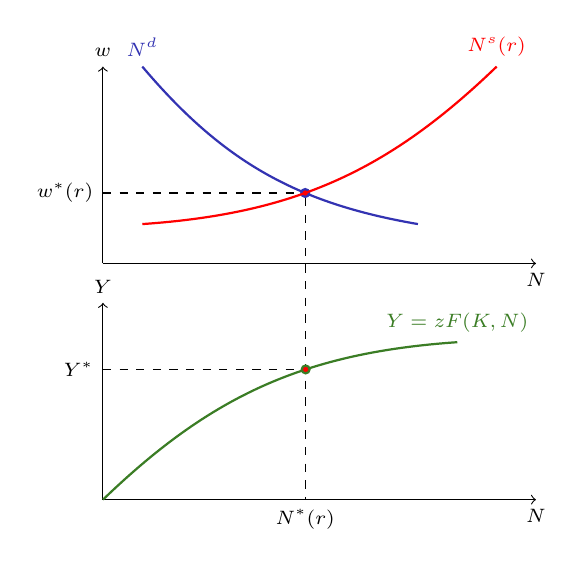
\begin{tikzpicture}
                \tikzstyle{every node}=[font=\scriptsize]
                \pgfmathsetmacro{\x}{5};
                \pgfmathsetmacro{\y}{2.5};
                % \draw[very thin,color=gray, step=0.1] (0,0) grid (\x, \y); % gray grid
                \draw[->, yshift = 3cm] (0,0) -- (\x + 0.5,0) node[below]{$N$} ;   % label x axis
                \draw[->, yshift = 3cm] (0,0) --  (0,\y) node[above]{$w$} ;   % label y axis
                \draw[thick, blue, yshift = 3cm]
                    (0.5, \y)
                    node[above]{$N^{d}$}
                    to[bend right=20]
                    node[pos=0.65,draw,fill=red,circle,inner sep=1pt] (a) {}
                    (4, 0.5);
                \draw[thick, red, yshift = 3cm]
                    (\x, \y)
                    node[above]{$N^{s}( r )$}
                    to[bend left=20]
                    (0.5, 0.5);
                \path (a); \pgfgetlastxy{\xcoord}{\ycoord};
                \coordinate (a_x) at (\xcoord, 0);
                \coordinate (a_y) at (0, \ycoord);

                \draw[dashed] (a_y) node[left]{$w^{*}( r )$} -- (a) -- (a_x) node[below]{$N^{*}( r )$};

                \draw[->] (0,0) -- (\x + 0.5,0) node[below]{$N$} ;   % label x axis
                \draw[->] (0,0) --  (0,\y) node[above]{$Y$} ;   % label y axis
                \draw[thick, OliveGreen]
                    (0, 0)
                    to[bend left=20]
                    node[pos=0.62,draw,fill=red,circle,inner sep=1pt] (b) {}
                    (\x-0.5, \y-0.5)
                    node[above]{$Y = zF(K, N)$};
                \path (b); \pgfgetlastxy{\xcoord}{\ycoord};
                \coordinate (b_x) at (\xcoord, 0);
                \coordinate (b_y) at (0, \ycoord);
                \draw[dashed] (b_y) node[left]{$Y^{*}$} -- (b) ;

            \end{tikzpicture}

        \end{column}
        \begin{column}{0.5\textwidth}
            \begin{itemize}
                \item $ r $ increases?
                \begin{itemize}
                    \item \textbf{N2} (consumer): $ N^{s}( r ) \uparrow  $ in $ r $ $ \Rightarrow  $ $ w \downarrow  $, $ N^{*}( r ) \uparrow  $
                    \item \textbf{firm}: $ \because MPN = w $, same
                \end{itemize}
                \item consumer wealth increases?
                \begin{itemize}
                    \item \textbf{N3} (consumer): $ N^{s}( r ) \downarrow \Rightarrow w \uparrow  $, $ N^{*}( r ) \downarrow  $
                    \item \textbf{firm}: nothing
                \end{itemize}
                \item Bottom chart: $ N^{*}( r ) \rightarrow Y^{*}( r ) $, \alert{output supply}!
            \end{itemize}
        \end{column}
    \end{columns}


\end{frame}



\begin{frame}{The Output Supply Curve}
\label{slide:The_Output_Supply_Curve}
    \begin{columns}
        \begin{column}{0.5\textwidth}
            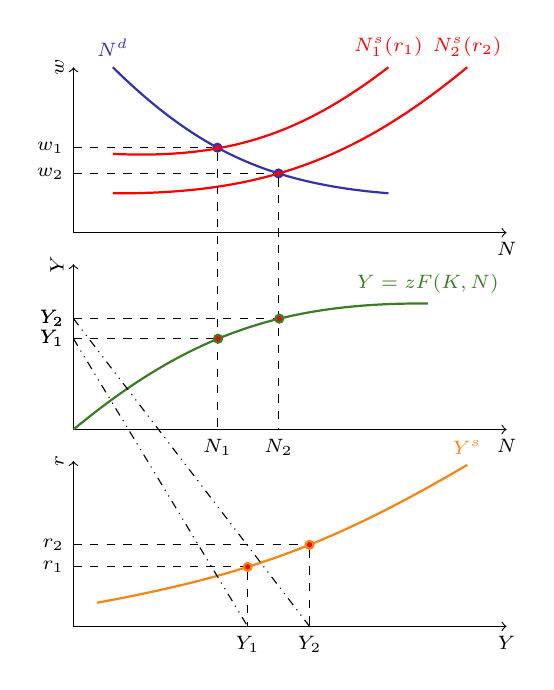
\begin{tikzpicture}
                \tikzstyle{every node}=[font=\scriptsize]
                \pgfmathsetmacro{\x}{5};
                \pgfmathsetmacro{\y}{2.1};
                % \draw[very thin,color=gray, step=1] (0,0) grid (\x, \y); % gray grid
                \draw[->, yshift = 5cm] (0,0) -- (\x + 0.5,0) node[below]{$N$} ;   % label x axis
                \draw[->, yshift = 5cm] (0,0) --  (0,\y) node[above, rotate=90]{$w$} ;   % label y axis
                \draw[thick, blue, yshift = 5cm]
                    (0.5, \y)
                    node[above]{$N^{d}$}
                    to[bend right=20]
                    node[pos=0.42,draw,fill=red,circle,inner sep=1pt] (a) {}
                    node[pos=0.65,draw,fill=red,circle,inner sep=1pt] (b) {}
                    (4, 0.5);
                \draw[thick, red, yshift = 5cm]
                    (\x-1, \y)
                    node[above]{$N_{1}^{s}( r_{1} )$}
                    to[bend left=20]
                    (0.5, 1);
                \draw[thick, red, yshift = 5cm]
                    (\x, \y)
                    node[above]{$N_{2}^{s}( r_{2} )$}
                    to[bend left=20]
                    (0.5, 0.5);
                \path (a); \pgfgetlastxy{\xcoord}{\ycoord};
                \coordinate (a_x) at (\xcoord, 2.5);
                \coordinate (a_y) at (0, \ycoord);
                \path (b); \pgfgetlastxy{\xcoord}{\ycoord};
                \coordinate (b_x) at (\xcoord, 2.5);
                \coordinate (b_y) at (0, \ycoord);

                \draw[dashed] (a_y) node[left]{$w_{1}$} -- (a) -- (a_x) node[below]{$N_{1}$};
                \draw[dashed] (b_y) node[left]{$w_{2}$} -- (b) -- (b_x) node[below]{$N_{2}$};

                \draw[->, yshift = 2.5cm] (0,0) -- (\x + 0.5,0) node[below]{$N$} ;   % label x axis
                \draw[->, yshift = 2.5cm] (0,0) --  (0,\y) node[above, rotate=90]{$Y$} ;   % label y axis

                \draw[thick, OliveGreen, yshift = 2.5cm]
                    (0, 0)
                    to[bend left=20]
                    node[pos=0.44,draw,fill=red,circle,inner sep=1pt] (c) {}
                    node[pos=0.62,draw,fill=red,circle,inner sep=1pt] (d) {}
                    (\x-0.5, \y-0.5)
                    node[above]{$Y = zF(K, N)$};
                \path (c); \pgfgetlastxy{\xcoord}{\ycoord};
                \coordinate (c_x) at (\xcoord, 2.5);
                \coordinate (c_y) at (0, \ycoord);
                \path (d); \pgfgetlastxy{\xcoord}{\ycoord};
                \coordinate (d_x) at (\xcoord, 2.5);
                \coordinate (d_y) at (0, \ycoord);
                \draw[dashed] (c_y) node[left]{$Y_{1}$} -- (c);
                \draw[dashed] (d_y) node[left]{$Y_{2}$} -- (d);

                \draw[->] (0,0) -- (\x + 0.5,0) node[below]{$Y$} ;   % label x axis
                \draw[->] (0,0) --  (0,\y) node[above, rotate=90]{$r$} ;   % label y axis

                \draw[thick, BurntOrange]
                    (\x, \y-0.05)
                    node[above]{$Y^{s}$}
                    to[bend left=10]
                    node[pos=0.44,draw,fill=red,circle,inner sep=1pt] (e) {}
                    node[pos=0.62,draw,fill=red,circle,inner sep=1pt] (f) {}
                    (0.3, 0.3);
                \path (e); \pgfgetlastxy{\xcoord}{\ycoord};
                \coordinate (e_x) at (\xcoord, 0);
                \coordinate (e_y) at (0, \ycoord);
                \path (f); \pgfgetlastxy{\xcoord}{\ycoord};
                \coordinate (f_x) at (\xcoord, 0);
                \coordinate (f_y) at (0, \ycoord);
                \draw[dash dot dot] (c_y) node[left]{$Y_{1}$} -- (f_x) ;
                \draw[dash dot dot] (d_y) node[left]{$Y_{2}$} -- (e_x) ;
                \draw[dashed] (f_y) node[left]{$r_{1}$} -- (f) -- (f_x) node[below]{$Y_{1}$};
                \draw[dashed] (e_y) node[left]{$r_{2}$} -- (e) -- (e_x) node[below]{$Y_{2}$};

            \end{tikzpicture}

        \end{column}
        \begin{column}{0.5\textwidth}
            Using our insight from labor market, we can repeat out analysis for any real interest rate $ r $
            \begin{itemize}
                \item Top: each $ r $ implies a different ``labor market equilibrium'', i.e., $ w $ \& $ N $
                \item Middle: each $ N( r ) $ yields production $ Y^{S}( r ) $
                \item Buttom: combined to show $ \displaystyle \frac{d Y^{S}}{dr} > 0 $
            \end{itemize}
        \end{column}
    \end{columns}
\end{frame}

\begin{frame}{Shifts in the Output Supply Curve}
\label{slide:Shifts_in_the_Output_Supply_Curve}
    How do changes in exogenous variables shift $ Y^{S}( r ) $? Consider 2 cases:
    \begin{enumerate}
        \item shift in lifetime wealth (for example, by gov’t spending or taxation)
        \item change in total factor productivity (TFP) or capital stock
        \begin{itemize}
            \item recall static model: with $ K $ fixed, these have the same effect
        \end{itemize}
    \end{enumerate}
    In each case, we can start our analysis with the current labor market.
\end{frame}

\begin{frame}{Wealth and Output Supply}
\label{slide:Wealth_and_Output_Supply}
    \begin{columns}
        \begin{column}{0.5\textwidth}
            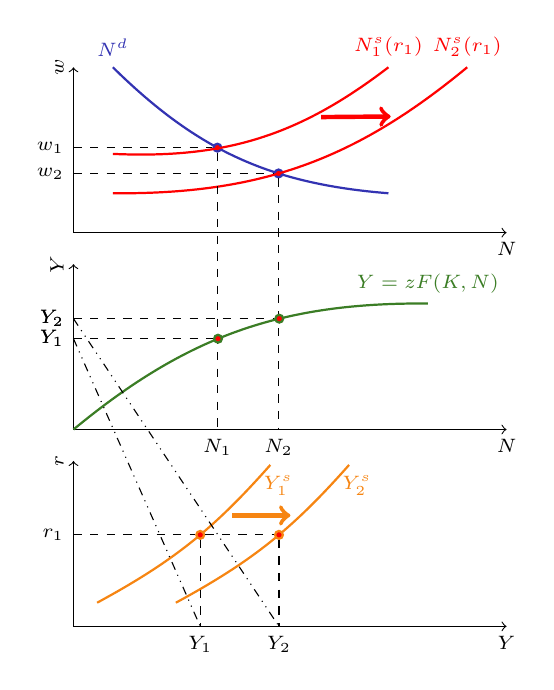
\begin{tikzpicture}
                \tikzstyle{every node}=[font=\scriptsize]
                \pgfmathsetmacro{\x}{5};
                \pgfmathsetmacro{\y}{2.1};
                % \draw[very thin,color=gray, step=1] (0,0) grid (\x, \y); % gray grid
                \draw[->, yshift = 5cm] (0,0) -- (\x + 0.5,0) node[below]{$N$} ;   % label x axis
                \draw[->, yshift = 5cm] (0,0) --  (0,\y) node[above, rotate=90]{$w$} ;   % label y axis
                \draw[thick, blue, yshift = 5cm]
                    (0.5, \y)
                    node[above]{$N^{d}$}
                    to[bend right=20]
                    node[pos=0.42,draw,fill=red,circle,inner sep=1pt] (a) {}
                    node[pos=0.65,draw,fill=red,circle,inner sep=1pt] (b) {}
                    (4, 0.5);
                \draw[thick, red, yshift = 5cm]
                    (\x-1, \y)
                    node[above]{$N_{1}^{s}( r_{1} )$}
                    to[bend left=20]
                    node[pos=0.3] (g) {}
                    (0.5, 1);
                \draw[thick, red, yshift = 5cm]
                    (\x, \y)
                    node[above]{$N_{2}^{s}( r_{1} )$}
                    to[bend left=20]
                    node[pos=0.2] (h) {}
                    (0.5, 0.5);
                \path (a); \pgfgetlastxy{\xcoord}{\ycoord};
                \coordinate (a_x) at (\xcoord, 2.5);
                \coordinate (a_y) at (0, \ycoord);
                \path (b); \pgfgetlastxy{\xcoord}{\ycoord};
                \coordinate (b_x) at (\xcoord, 2.5);
                \coordinate (b_y) at (0, \ycoord);

                \draw[dashed] (a_y) node[left]{$w_{1}$} -- (a) -- (a_x) node[below]{$N_{1}$};
                \draw[dashed] (b_y) node[left]{$w_{2}$} -- (b) -- (b_x) node[below]{$N_{2}$};
                \draw[ultra thick, red, ->] (g) -- (h) ;

                \draw[->, yshift = 2.5cm] (0,0) -- (\x + 0.5,0) node[below]{$N$} ;   % label x axis
                \draw[->, yshift = 2.5cm] (0,0) --  (0,\y) node[above, rotate=90]{$Y$} ;   % label y axis

                \draw[thick, OliveGreen, yshift = 2.5cm]
                    (0, 0)
                    to[bend left=20]
                    node[pos=0.44,draw,fill=red,circle,inner sep=1pt] (c) {}
                    node[pos=0.62,draw,fill=red,circle,inner sep=1pt] (d) {}
                    (\x-0.5, \y-0.5)
                    node[above]{$Y = zF(K, N)$};
                \path (c); \pgfgetlastxy{\xcoord}{\ycoord};
                \coordinate (c_x) at (\xcoord, 2.5);
                \coordinate (c_y) at (0, \ycoord);
                \path (d); \pgfgetlastxy{\xcoord}{\ycoord};
                \coordinate (d_x) at (\xcoord, 2.5);
                \coordinate (d_y) at (0, \ycoord);
                \draw[dashed] (c_y) node[left]{$Y_{1}$} -- (c);
                \draw[dashed] (d_y) node[left]{$Y_{2}$} -- (d);

                \draw[->] (0,0) -- (\x + 0.5,0) node[below]{$Y$} ;   % label x axis
                \draw[->] (0,0) --  (0,\y) node[above, rotate=90]{$r$} ;   % label y axis

                \draw[thick, BurntOrange]
                    (\x/2, \y-0.05)
                    node[below, xshift = 0.1cm]{$Y_{1}^{s}$}
                    to[bend left=10]
                    node[pos=0.44,draw,fill=red,circle,inner sep=1pt] (e) {}
                    node[pos=0.3] (i) {}
                    (0.3, 0.3);
                \draw[thick, BurntOrange, xshift = 1cm]
                    (\x/2, \y-0.05)
                    node[below, xshift = 0.1cm]{$Y_{2}^{s}$}
                    to[bend left=10]
                    node[pos=0.44,draw,fill=red,circle,inner sep=1pt] (f) {}
                    node[pos=0.3] (j) {}
                    (0.3, 0.3);
                \path (e); \pgfgetlastxy{\xcoord}{\ycoord};
                \coordinate (e_x) at (\xcoord, 0);
                \coordinate (e_y) at (0, \ycoord);
                \path (f); \pgfgetlastxy{\xcoord}{\ycoord};
                \coordinate (f_x) at (\xcoord, 0);
                \coordinate (f_y) at (0, \ycoord);
                \draw[dash dot dot] (c_y) node[left]{$Y_{1}$} -- (e_x) ;
                \draw[dash dot dot] (d_y) node[left]{$Y_{2}$} -- (f_x) ;
                \draw[dashed] (e_y) node[left]{$r_{1}$} -- (e) -- (e_x) node[below]{$Y_{1}$};
                \draw[dashed] (e) -- (f) -- (f_x) node[below]{$Y_{2}$};
                \draw[ultra thick, BurntOrange, ->] (i) -- (j) ;

            \end{tikzpicture}

        \end{column}
        \begin{column}{0.5\textwidth}
            Suppose $ G \uparrow  $ or $ G' \uparrow  $.
            \begin{itemize}
                \item gov. budget: $ T \uparrow  $ or $ T' \uparrow  $
                \item consumer budget: $ we \downarrow  $
                \item \textbf{N3}: $ \displaystyle d N^{S} / d ( we ) < 0 $, $ N^{S}( r ) \uparrow  $ (shift to the right, top panel)
                \item Middle: $ N\uparrow  $ $ \Rightarrow  $ $ Y^{S} \uparrow  $
                \item bottom: combine, get rightward shift in output supply
            \end{itemize}
        \end{column}
    \end{columns}
\end{frame}

\begin{frame}{TFP / Capital and Output Supply}
\label{slide:TFP___Capital_and_Output_Supply}
    \begin{columns}
        \begin{column}{0.5\textwidth}

            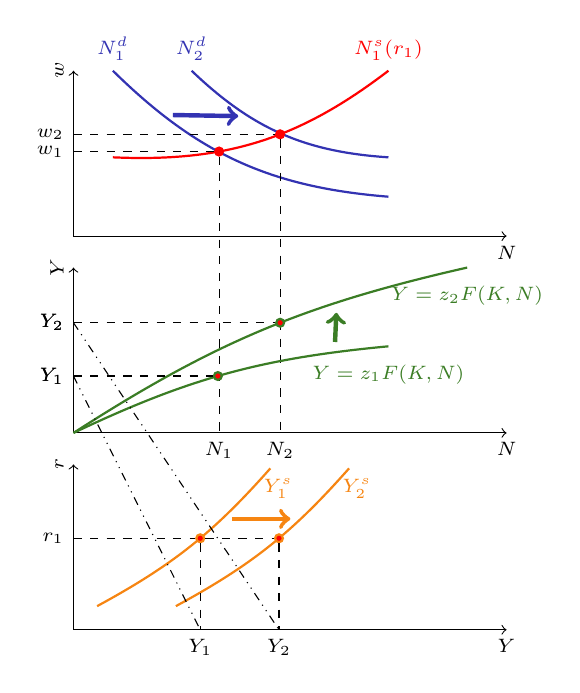
\begin{tikzpicture}
                \tikzstyle{every node}=[font=\scriptsize]
                \pgfmathsetmacro{\x}{5};
                \pgfmathsetmacro{\y}{2.1};
                % \draw[very thin,color=gray, step=1] (0,0) grid (\x, \y); % gray grid
                \draw[->, yshift = 5cm] (0,0) -- (\x + 0.5,0) node[below]{$N$} ;   % label x axis
                \draw[->, yshift = 5cm] (0,0) --  (0,\y) node[above, rotate=90]{$w$} ;   % label y axis
                \draw[thick, blue, yshift = 5cm]
                    (0.5, \y)
                    node[above]{$N_{1}^{d}$}
                    to[bend right=20]
                    node[pos=0.2] (aa) {}
                    (4, 0.5);
                \draw[thick, blue, yshift = 5cm]
                    (1.5, \y)
                    node[above]{$N_{2}^{d}$}
                    to[bend right=20]
                    node[pos=0.32] (bb) {}
                    (4, 1);
                \draw[thick, red, yshift = 5cm]
                    (\x-1, \y)
                    node[above]{$N_{1}^{s}( r_{1} )$}
                    to[bend left=20]
                    node[pos=0.42,draw,fill=red,circle,inner sep=1pt] (a) {}
                    node[pos=0.65,draw,fill=red,circle,inner sep=1pt] (b) {}
                    (0.5, 1);
                \path (a); \pgfgetlastxy{\xcoord}{\ycoord};
                \coordinate (a_x) at (\xcoord, 2.5);
                \coordinate (a_y) at (0, \ycoord);
                \path (b); \pgfgetlastxy{\xcoord}{\ycoord};
                \coordinate (b_x) at (\xcoord, 2.5);
                \coordinate (b_y) at (0, \ycoord);

                \draw[dashed] (a_y) node[left]{$w_{2}$} -- (a) -- (a_x) node[below]{$N_{2}$};
                \draw[dashed] (b_y) node[left]{$w_{1}$} -- (b) -- (b_x) node[below]{$N_{1}$};
                \draw[ultra thick, blue, ->] (aa) -- (bb);

                \draw[->, yshift = 2.5cm] (0,0) -- (\x + 0.5,0) node[below]{$N$} ;   % label x axis
                \draw[->, yshift = 2.5cm] (0,0) --  (0,\y) node[above, rotate=90]{$Y$} ;   % label y axis

                \draw[thick, OliveGreen, yshift = 2.5cm]
                    (0, 0)
                    to[bend left=10]
                    node[pos=0.47,draw,fill=red,circle,inner sep=1pt] (c) {}
                    node[pos=0.85] (cc) {}
                    % node[pos=0.62,draw,fill=red,circle,inner sep=1pt] (d) {}
                    (\x-1, \y-1)
                    node[below, yshift = -0.1cm]{$Y = z_{1}F(K, N)$};
                \draw[thick, OliveGreen, yshift = 2.5cm]
                    (0, 0)
                    to[bend left=10]
                    % node[pos=0.44,draw,fill=red,circle,inner sep=1pt] (c) {}
                    node[pos=0.55,draw,fill=red,circle,inner sep=1pt] (d) {}
                    node[pos=0.7] (dd) {}
                    (\x, \y)
                    node[below, yshift = -0.1cm]{$Y = z_{2}F(K, N)$};
                \path (c); \pgfgetlastxy{\xcoord}{\ycoord};
                \coordinate (c_x) at (\xcoord, 2.5);
                \coordinate (c_y) at (0, \ycoord);
                \path (d); \pgfgetlastxy{\xcoord}{\ycoord};
                \coordinate (d_x) at (\xcoord, 2.5);
                \coordinate (d_y) at (0, \ycoord);
                \draw[dashed] (c_y) node[left]{$Y_{1}$} -- (c);
                \draw[dashed] (d_y) node[left]{$Y_{2}$} -- (d);
                \draw[ultra thick, OliveGreen, ->] (cc) -- (dd);

                \draw[->] (0,0) -- (\x + 0.5,0) node[below]{$Y$} ;   % label x axis
                \draw[->] (0,0) --  (0,\y) node[above, rotate=90]{$r$} ;   % label y axis

                \draw[thick, BurntOrange]
                    (\x/2, \y-0.05)
                    node[below, xshift = 0.1cm]{$Y_{1}^{s}$}
                    to[bend left=10]
                    node[pos=0.44,draw,fill=red,circle,inner sep=1pt] (e) {}
                    node[pos=0.3] (i) {}
                    (0.3, 0.3);
                \draw[thick, BurntOrange, xshift = 1cm]
                    (\x/2, \y-0.05)
                    node[below, xshift = 0.1cm]{$Y_{2}^{s}$}
                    to[bend left=10]
                    node[pos=0.44,draw,fill=red,circle,inner sep=1pt] (f) {}
                    node[pos=0.3] (j) {}
                    (0.3, 0.3);
                \path (e); \pgfgetlastxy{\xcoord}{\ycoord};
                \coordinate (e_x) at (\xcoord, 0);
                \coordinate (e_y) at (0, \ycoord);
                \path (f); \pgfgetlastxy{\xcoord}{\ycoord};
                \coordinate (f_x) at (\xcoord, 0);
                \coordinate (f_y) at (0, \ycoord);
                \draw[dash dot dot] (c_y) node[left]{$Y_{1}$} -- (e_x) ;
                \draw[dash dot dot] (d_y) node[left]{$Y_{2}$} -- (f_x) ;
                \draw[dashed] (e_y) node[left]{$r_{1}$} -- (e) -- (e_x) node[below]{$Y_{1}$};
                \draw[dashed] (e) -- (f) -- (f_x) node[below]{$Y_{2}$};
                \draw[ultra thick, BurntOrange, ->] (i) -- (j) ;

            \end{tikzpicture}
        \end{column}
        \begin{column}{0.5\textwidth}
            Suppose TFP $ z \uparrow  $.
            \begin{itemize}
                \item \textbf{firm optimality}: $ MPN = z D_{N}F( \cdot ) \uparrow  $ $ \Rightarrow  $ $ N^{d} \uparrow  $
                \item Top: $ N^{d} $ shifts out $ \Rightarrow  $ $ w^{*} \uparrow, N^{*} \uparrow  $
                \item Middle: production fcn shifts up, $ \because z \uparrow $
                \item Bottom: combine, outward shift in output supply
            \end{itemize}
        \end{column}
    \end{columns}
\end{frame}

\begin{frame}{Summary: Current Labor Market}
\label{slide:Summary__Current_Labor_Market}
    We have constructed most of the model!
    \begin{itemize}
        \item \alert{labor market clearing}, \textit{conditional on} the interest rate
        \item trace through production function to get \alert{output supply curve}
    \end{itemize}
    Now we need to determine the \alert{equilibrium interest rate}, $ r^{*} $.
    \begin{itemize}
        \item pair the \alert{output supply curve} with the \textbf{output demand curve}
        \item who demands goods today, and how much?
        \begin{itemize}
            \item consumer: consumption $ C^{d}( r, Y ) $
            \item firm: investment $ I^{d}( r ) $
            \item government: expenditures $ G $
            \item use GDP accounting to get aggregate demand for goods
        \end{itemize}
    \end{itemize}
\end{frame}



\begin{frame}{Current Goods Demand}
\label{slide:Current_Goods_Demand}
    \begin{columns}
        \begin{column}{0.5\textwidth}
            \begin{center}
                \scriptsize
                Figure 11.18  The Demand for Current Goods
            \end{center}
            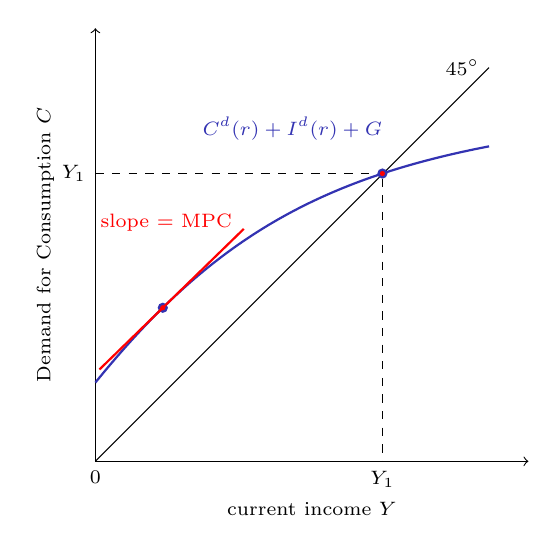
\begin{tikzpicture}[domain=0:5]
                \tikzstyle{every node}=[font=\scriptsize]
                \pgfmathsetmacro{\x}{5};
                \pgfmathsetmacro{\y}{5};
                % \draw[very thin,color=gray, step=0.1] (0,0) grid (\x, \y); % gray grid
                \draw[->] (0,0) node[below]{ $ 0 $  } -- node[below, yshift = -0.4cm]{current income $Y$} (\x + 0.5,0) ;   % label x axis
                \draw[->] (0,0) -- node[above, rotate=90, yshift = 0.4cm]{Demand for Consumption $ C $} (0,\y + 0.5) ;   % label y axis
                \draw[black] plot (\x, \x) node[left]{$45^{\circ}$};
                \draw[thick, blue, yshift = -1cm] (0, 2)
                    to[bend left=20]
                    node[pos=0.2,draw,fill=red,circle,inner sep=1pt] (a) {}
                    node[pos=0.21] (b) {}
                    node[pos=0.78,draw,fill=red,circle,inner sep=1pt] (c) {}
                    (5, 5) node[below, xshift = -2.5cm, yshift = 0.5cm]{$C^{d}( r ) + I^{d}( r ) + G$};
                \draw[shorten >=-1cm, shorten <=-1.5cm, thick, red] (a) -- (b) node[above, yshift=.8cm]{slope $=$ MPC};
                \path (c); \pgfgetlastxy{\xcoord}{\ycoord};
                \coordinate (c_x) at (\xcoord, 0);
                \coordinate (c_y) at (0, \ycoord);
                \draw[dashed] (c_y) node[left]{$Y_{1}$}  -- (c) -- (c_x) node[below]{$Y_{1}$};
            \end{tikzpicture}
        \end{column}
        \begin{column}{0.5\textwidth}
            $ \displaystyle D( r, Y ) = C^{d} ( r, Y ) + I^{d}( r ) + G $
            \begin{itemize}
                \item plot $ D( r, Y ) $ on $ y $-axis, $ Y $ on $ x $-axis
                \item $ C^{d} $ depends on wealth:
                    $ \displaystyle we = wN + \pi - T + \frac{w'N' + \pi' - T'}{1+r} $,
                    which depends on income.
                \item Not true for $ I $ and $ G $
                \begin{itemize}
                    \item $ MPC < 1 $: flatter than $ 45^{\circ} $ line
                    \item $ MPC $ diminishing: concave
                    \item combine: cross $ 45^{\circ} $ line at $ Y^{d}( r ) $
                \end{itemize}
            \end{itemize}
        \end{column}
    \end{columns}
\end{frame}

\begin{frame}{Constructing Output Demand}
\label{slide:Constructing_Output_Demand}
    \begin{columns}
        \begin{column}{0.5\textwidth}
            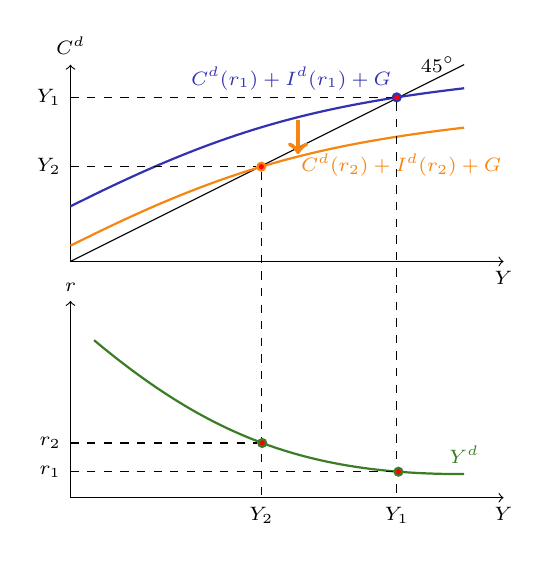
\begin{tikzpicture}[domain=0:5]
                \tikzstyle{every node}=[font=\scriptsize]
                \pgfmathsetmacro{\x}{5};
                \pgfmathsetmacro{\y}{2.5};
                % \draw[very thin,color=gray, step=0.1] (0,0) grid (\x, \y); % gray grid

                \draw[->, yshift = 3cm] (0,0) -- (\x + 0.5,0) node[below]{$Y$} ;   % label x axis
                \draw[->, yshift = 3cm] (0,0) --  (0,\y) node[above]{$C^{d}$} ;   % label y axis
                \draw[black, yshift = 3cm] plot (\x, \x/2) node[left]{$45^{\circ}$};

                \draw[thick, blue, yshift = 1.7cm] (0, 2)
                    to[bend left=10]
                    node[pos=0.85,draw,fill=red,circle,inner sep=1pt] (c) {}
                    node[pos=0.6] (cc) {}
                    (5, 3.5) node[below, yshift = 0.4cm, xshift = -2.2cm]{$C^{d}( r_{1} ) + I^{d}( r_{1} ) + G$};
                \draw[thick, BurntOrange, yshift = 1.2cm] (0, 2)
                    to[bend left=10]
                    node[pos=0.5,draw,fill=red,circle,inner sep=1pt] (f) {}
                    node[pos=0.6] (ff) {}
                    (5, 3.5) node[below, xshift = -0.8cm, yshift = -0.2cm]{$C^{d}( r_{2} ) + I^{d}( r_{2} ) + G$};

                \path (c); \pgfgetlastxy{\xcoord}{\ycoord};
                \coordinate (c_x) at (\xcoord, 0);
                \coordinate (c_y) at (0, \ycoord);
                \draw[dashed] (c_y) node[left]{$Y_{1}$}  -- (c) -- (c_x) node[below]{$Y_{1}$};
                \path (f); \pgfgetlastxy{\xcoord}{\ycoord};
                \coordinate (f_x) at (\xcoord, 0);
                \coordinate (f_y) at (0, \ycoord);
                \draw[dashed] (f_y) node[left]{$Y_{2}$}  -- (f) -- (f_x) node[below]{$Y_{2}$};
                \draw[ultra thick, BurntOrange, ->, shorten >= -0.1cm, shorten <= -0.1cm] (cc) -- (ff);

                \draw[->] (0,0) -- (\x + 0.5,0) node[below]{$Y$} ;   % label x axis
                \draw[->] (0,0) --  (0,\y) node[above]{$r$} ;   % label y axis
                \draw[thick, OliveGreen]
                    (0.3, \y-0.5)
                    to[bend right=20]
                    node[pos=0.49,draw,fill=red,circle,inner sep=1pt] (b) {}
                    node[pos=0.85,draw,fill=red,circle,inner sep=1pt] (d) {}
                    (\x, 0.3)
                    node[above]{$Y^{d}$};
                \path (b); \pgfgetlastxy{\xcoord}{\ycoord};
                \coordinate (b_x) at (\xcoord, 0);
                \coordinate (b_y) at (0, \ycoord);
                \path (d); \pgfgetlastxy{\xcoord}{\ycoord};
                \coordinate (d_x) at (\xcoord, 0);
                \coordinate (d_y) at (0, \ycoord);
                \draw[dashed] (b_y) node[left]{$r_{2}$} -- (b) ;
                \draw[dashed] (d_y) node[left]{$r_{1}$} -- (d) ;

            \end{tikzpicture}

        \end{column}
        \begin{column}{0.5\textwidth}
            How different $ r $ affect output demand?
            \begin{itemize}
                \item \textbf{C2} (consumer): \alert{$C^{d}( r ) \downarrow $} if $ r \uparrow  $(substitution effect dominates)
                \item \textbf{firm}: optimal investment schedule ($r = MPK' - \delta$), $ r \uparrow  $ $ \Rightarrow  $ $ MPK' \uparrow  $ $ \Rightarrow  $ $ I^{d} \downarrow  $
                \item \textbf{gov}: no change, $ \because G $ exogenous
                \item Combine:
                \begin{enumerate}
                    \item intersection with $ 45^{\circ} $ line is lower
                    \item \alert{output demand curve} $ Y^{d} $ downward slope
                \end{enumerate}
            \end{itemize}
        \end{column}
    \end{columns}
\end{frame}

\begin{frame}{Constructing Output Demand (Cont.)}
\label{slide:Constructing_Output_Demand__Cont__}
    \begin{columns}
        \begin{column}{0.5\textwidth}
            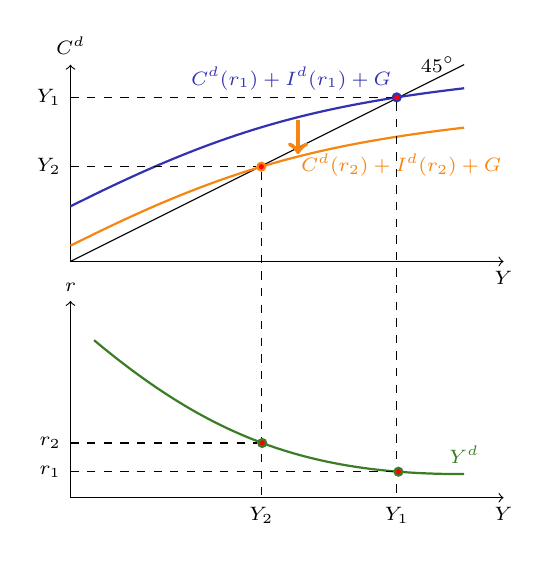
\begin{tikzpicture}[domain=0:5]
                \tikzstyle{every node}=[font=\scriptsize]
                \pgfmathsetmacro{\x}{5};
                \pgfmathsetmacro{\y}{2.5};
                % \draw[very thin,color=gray, step=0.1] (0,0) grid (\x, \y); % gray grid

                \draw[->, yshift = 3cm] (0,0) -- (\x + 0.5,0) node[below]{$Y$} ;   % label x axis
                \draw[->, yshift = 3cm] (0,0) --  (0,\y) node[above]{$C^{d}$} ;   % label y axis
                \draw[black, yshift = 3cm] plot (\x, \x/2) node[left]{$45^{\circ}$};

                \draw[thick, blue, yshift = 1.7cm] (0, 2)
                    to[bend left=10]
                    node[pos=0.85,draw,fill=red,circle,inner sep=1pt] (c) {}
                    node[pos=0.6] (cc) {}
                    (5, 3.5) node[below, yshift = 0.4cm, xshift = -2.2cm]{$C^{d}( r_{1} ) + I^{d}( r_{1} ) + G$};
                \draw[thick, BurntOrange, yshift = 1.2cm] (0, 2)
                    to[bend left=10]
                    node[pos=0.5,draw,fill=red,circle,inner sep=1pt] (f) {}
                    node[pos=0.6] (ff) {}
                    (5, 3.5) node[below, xshift = -0.8cm, yshift = -0.2cm]{$C^{d}( r_{2} ) + I^{d}( r_{2} ) + G$};

                \path (c); \pgfgetlastxy{\xcoord}{\ycoord};
                \coordinate (c_x) at (\xcoord, 0);
                \coordinate (c_y) at (0, \ycoord);
                \draw[dashed] (c_y) node[left]{$Y_{1}$}  -- (c) -- (c_x) node[below]{$Y_{1}$};
                \path (f); \pgfgetlastxy{\xcoord}{\ycoord};
                \coordinate (f_x) at (\xcoord, 0);
                \coordinate (f_y) at (0, \ycoord);
                \draw[dashed] (f_y) node[left]{$Y_{2}$}  -- (f) -- (f_x) node[below]{$Y_{2}$};
                \draw[ultra thick, BurntOrange, ->, shorten >= -0.1cm, shorten <= -0.1cm] (cc) -- (ff);

                \draw[->] (0,0) -- (\x + 0.5,0) node[below]{$Y$} ;   % label x axis
                \draw[->] (0,0) --  (0,\y) node[above]{$r$} ;   % label y axis
                \draw[thick, OliveGreen]
                    (0.3, \y-0.5)
                    to[bend right=20]
                    node[pos=0.49,draw,fill=red,circle,inner sep=1pt] (b) {}
                    node[pos=0.85,draw,fill=red,circle,inner sep=1pt] (d) {}
                    (\x, 0.3)
                    node[above]{$Y^{d}$};
                \path (b); \pgfgetlastxy{\xcoord}{\ycoord};
                \coordinate (b_x) at (\xcoord, 0);
                \coordinate (b_y) at (0, \ycoord);
                \path (d); \pgfgetlastxy{\xcoord}{\ycoord};
                \coordinate (d_x) at (\xcoord, 0);
                \coordinate (d_y) at (0, \ycoord);
                \draw[dashed] (b_y) node[left]{$r_{2}$} -- (b) ;
                \draw[dashed] (d_y) node[left]{$r_{1}$} -- (d) ;

            \end{tikzpicture}

        \end{column}
        \begin{column}{0.5\textwidth}
            Combine:
            \begin{enumerate}
                \item intersection with $ 45^{\circ} \downarrow $
                \item \alert{output demand curve} $ Y^{d} $ downward sloping
            \end{enumerate}
            $ Y^{d}( r ) $ shift to the right if
            \begin{enumerate}
                \item present value of taxes $ \downarrow  $ $ \Rightarrow  $ $ C^{d} \uparrow  $
                \item future income $ \uparrow  $ $ \Rightarrow  $ $ C^{d} \uparrow  $
                \item future TFP $ \uparrow  $ $ \Rightarrow  $ $ I^{d} \uparrow $
                \item current capital $ \downarrow  $ $ \Rightarrow  $ $ I^{d} \uparrow  $
            \end{enumerate}
            Other changes (e.g., current TFP) are ambiguous in general!
        \end{column}
    \end{columns}
\end{frame}


\begin{frame}{Competitive Equilibrium}
\label{slide:Competitive_Equilibrium}
    \begin{center}
        \scriptsize Figure 11.21  The Complete Real Intertemporal Model
    \end{center}
    \begin{columns}
        \begin{column}{0.5\textwidth}
            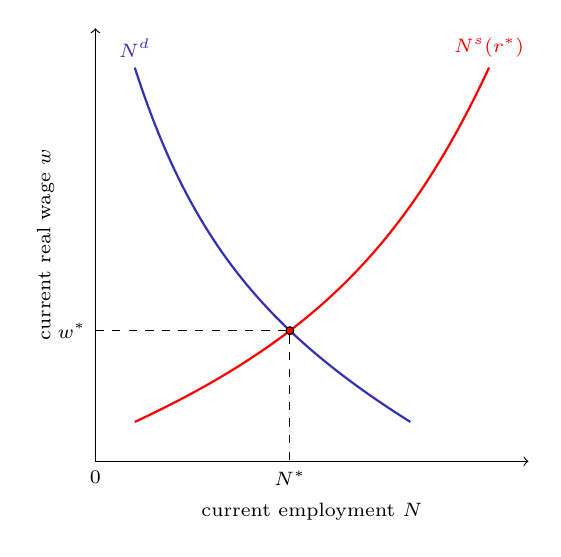
\begin{tikzpicture}[domain=0:5]
                \tikzstyle{every node}=[font=\scriptsize]
                \pgfmathsetmacro{\x}{5};
                \pgfmathsetmacro{\y}{5};
                % \draw[very thin,color=gray, step=0.1] (0,0) grid (\x, \y); % gray grid
                \draw[->] (0,0) node[below]{ $ 0 $  } -- node[below, yshift = -0.4cm]{current employment $ N $} (\x + 0.5,0) ;   % label x axis
                \draw[->] (0,0) -- node[above, rotate=90, yshift = 0.4cm]{current real wage $w$} (0,\y + 0.5) ;   % label y axis
                \draw[thick, red, name path = aa]
                    (\x, \y)
                    node[above]{$N^{s}( r^{*} )$}
                    to[bend left=20]
                    (0.5, 0.5);
                \draw[thick, blue, name path = bb]
                    (0.5, \y)
                    node[above]{$N^{d}$}
                    to[bend right=20]
                    (4, 0.5);
                \path[name intersections={of=aa and bb, by=b}];
                \node[draw,fill=red,circle,inner sep=1pt] at (b) {};
                \path (b); \pgfgetlastxy{\xcoord}{\ycoord};
                \coordinate (b_x) at (\xcoord, 0);
                \coordinate (b_y) at (0, \ycoord);
                \draw[dashed] (b_y) node[left]{$w^{*}$}  -- (b) -- (b_x) node[below]{$N^{*}$};

            \end{tikzpicture}
        \end{column}
        \begin{column}{0.5\textwidth}

            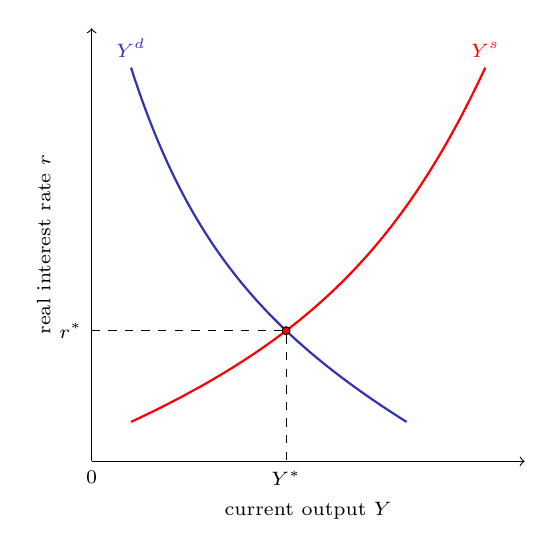
\begin{tikzpicture}[domain=0:5]
                \tikzstyle{every node}=[font=\scriptsize]
                \pgfmathsetmacro{\x}{5};
                \pgfmathsetmacro{\y}{5};
                % \draw[very thin,color=gray, step=0.1] (0,0) grid (\x, \y); % gray grid
                \draw[->] (0,0) node[below]{ $ 0 $  } -- node[below, yshift = -0.4cm]{current output $ Y $} (\x + 0.5,0) ;   % label x axis
                \draw[->] (0,0) -- node[above, rotate=90, yshift = 0.4cm]{real interest rate $r$} (0,\y + 0.5) ;   % label y axis
                \draw[thick, red, name path = aa]
                    (\x, \y)
                    node[above]{$Y^{s}$}
                    to[bend left=20]
                    (0.5, 0.5);
                \draw[thick, blue, name path = bb]
                    (0.5, \y)
                    node[above]{$Y^{d}$}
                    to[bend right=20]
                    (4, 0.5);
                \path[name intersections={of=aa and bb, by=a}];
                \node[draw,fill=red,circle,inner sep=1pt] at (a) {};
                \path (a); \pgfgetlastxy{\xcoord}{\ycoord};
                \coordinate (a_x) at (\xcoord, 0);
                \coordinate (a_y) at (0, \ycoord);
                \draw[dashed] (a_y) node[left]{$r^{*}$}  -- (a) -- (a_x) node[below]{$Y^{*}$};

            \end{tikzpicture}
        \end{column}
    \end{columns}
\end{frame}
\end{document}

